%%%%%%%%%%%%%%%%%%%%%%%%%%%%%%%%%%%%%%%%%
% Beamer Presentation
% LaTeX Template
% Version 1.0 (10/11/12)
%
% This template has been downloaded from:
% http://www.LaTeXTemplates.com
%
% License:
% CC BY-NC-SA 3.0 (http://creativecommons.org/licenses/by-nc-sa/3.0/)
%
%%%%%%%%%%%%%%%%%%%%%%%%%%%%%%%%%%%%%%%%%

%----------------------------------------------------------------------------------------
%	PACKAGES AND THEMES
%----------------------------------------------------------------------------------------

\documentclass{beamer}

\mode<presentation> {

% The Beamer class comes with a number of default slide themes
% which change the colors and layouts of slides. Below this is a list
% of all the themes, uncomment each in turn to see what they look like.

%\usetheme{default}
%\usetheme{AnnArbor}
%\usetheme{Antibes}
%\usetheme{Bergen}
%\usetheme{Berkeley}
%\usetheme{Berlin}
%\usetheme{Boadilla}
%\usetheme{CambridgeUS}
%\usetheme{Copenhagen}
%\usetheme{Darmstadt}
%\usetheme{Dresden}
%\usetheme{Frankfurt}
%\usetheme{Goettingen}
%\usetheme{Hannover}
%\usetheme{Ilmenau}
%\usetheme{JuanLesPins}
%\usetheme{Luebeck}
\usetheme{Madrid}
%\usetheme{Malmoe}
%\usetheme{Marburg}
%\usetheme{Montpellier}
%\usetheme{PaloAlto}
%\usetheme{Pittsburgh}
%\usetheme{Rochester}
%\usetheme{Singapore}
%\usetheme{Szeged}
%\usetheme{Warsaw}

% As well as themes, the Beamer class has a number of color themes
% for any slide theme. Uncomment each of these in turn to see how it
% changes the colors of your current slide theme.

%\usecolortheme{albatross}
%\usecolortheme{beaver}
%\usecolortheme{beetle}
%\usecolortheme{crane}
%\usecolortheme{dolphin}
%\usecolortheme{dove}
%\usecolortheme{fly}
%\usecolortheme{lily}
%\usecolortheme{orchid}
%\usecolortheme{rose}
%\usecolortheme{seagull}
%\usecolortheme{seahorse}
%\usecolortheme{whale}
%\usecolortheme{wolverine}

%\setbeamertemplate{footline} % To remove the footer line in all slides uncomment this line
%\setbeamertemplate{footline}[page number] % To replace the footer line in all slides with a simple slide count uncomment this line

\setbeamertemplate{navigation symbols}{} % To remove the navigation symbols from the bottom of all slides uncomment this line
}

\usepackage{graphicx} % Allows including images
\usepackage{booktabs} % Allows the use of \toprule, \midrule and \bottomrule in tables
\usepackage[utf8]{inputenc}

\usepackage{hyperref}
\definecolor{links}{HTML}{3578cc}
\hypersetup{colorlinks,linkcolor=,urlcolor=links}

%----------------------------------------------------------------------------------------
%	TITLE PAGE
%----------------------------------------------------------------------------------------

\title[Cytokine Graph DB]{ Cytokine Graph Database } % The short title appears at the bottom of every slide, the full title is only on the title page

\author{ Borna Bešić, Dilmurat Yusuf } % Your name
\institute[] % Your institution as it will appear on the bottom of every slide, may be shorthand to save space
{
Bioinformatics Group \\
\medskip
Albert-Ludwigs-Universität, Freiburg  % Your institution for the title page
}
\date{\today} % Date, can be changed to a custom date

\begin{document}

\begin{frame}
\titlepage % Print the title page as the first slide
\end{frame}

%----------------------------------------------------------------------------------------
%	PRESENTATION SLIDES
%----------------------------------------------------------------------------------------

\AtBeginSection[]{
    \begin{frame}{Overview}
        \tableofcontents[currentsection, hideothersubsections]
    \end{frame}
}

%------------------------------------------------
\section{Introduction} % Sections can be created in order to organize your presentation into discrete blocks, all sections and subsections are automatically printed in the table of contents as an overview of the talk
%------------------------------------------------

\begin{frame}{What do we want?}
\begin{itemize}
    \item Easier access to data
    \begin{itemize}
        \item More flexible searches
        \item Faster queries
        \item Dynamic user interfaces
    \end{itemize}
    \vfill
    \item Associated data in one place
    \begin{itemize}
        \item Unification of databases
    \end{itemize}
    \vfill
    \item This leads to
    \begin{itemize}
        \item Accessible protein - disease data
        \item Faster drug discovery
    \end{itemize}
    \vfill
    \item ...
\end{itemize}
\end{frame}
%------------------------------------------------

\begin{frame}{STRING}
    \begin{itemize}
        \item Database of known and predicted protein-protein interactions
        \vfill
        \item 7 score channels $ \rightarrow $ combined score
        \begin{enumerate}
            \item Experiments
            \item Database
            \item Textmining
            \item Co-expression
            \item Neighbourhood
            \item Fusion
            \item Co-occurence
        \end{enumerate}
        \vfill
        \item Best overall performance for gene set recovery by propagation (\href{https://www.ncbi.nlm.nih.gov/pubmed/29605183}{Huang et al., Systematic Evaluation of Molecular Networks for Discovery of Disease Genes, Cell Systems})
        \vfill
        \item Full database dumps available for download: 512.8 GB (compressed)
    \end{itemize}
\end{frame}

\begin{frame}{Graph databases}
    \begin{itemize}
        \item Nodes
        \item \textbf{Directed} edges / relationships
        \item Properties
    \end{itemize}
    \begin{figure}
        \centering
        \includegraphics[width=0.75\linewidth]{graph_database.png}
    \end{figure}
\end{frame}

\begin{frame}{Neo4j \& Cypher}
\begin{block}{Example of a Cypher query}
MATCH (:person \{ name: "Alan" \})-[p:PURCHASED]-\textgreater(b:book) \\
RETURN p.date, b
\end{block}
\begin{itemize}
    \item Pros:
    \begin{itemize}
        \item Outperforming RDBMS for associative data
        \item No redundancy
        \item Easier to change the design
    \end{itemize}
    \vfill
    \item Cons:
    \begin{itemize}
        \item Not standard; new query language (Cypher)
        \item Harder to do summing queries and max queries efficiently
    \end{itemize}
\end{itemize}
\end{frame}

\begin{frame}{Why Neo4j?}
    \begin{figure}
        \centering
        \includegraphics[width=0.7\linewidth]{graph-dbs-benchmark.png}
        \caption{\href{https://www.ncbi.nlm.nih.gov/pmc/articles/PMC3842757/}{Have CT, Jensen LJ. Are graph databases ready for bioinformatics?}}
    \end{figure}
\end{frame}

\begin{frame}
\frametitle{Cytokines}
\begin{itemize}
    \item Molecular messengers between cells
    \item Interact with cells of the immune system
    \item Regulate the body's response to disease and infection
    \item Mediate normal cellular processes in the body
\end{itemize}
\begin{figure}
    \centering
    \includegraphics[width=0.5\linewidth]{cytokines.jpg}
\end{figure}
\end{frame}

%------------------------------------------------

\section{Methodology}
\begin{frame}{Sources of data}
\begin{columns}[c] % The "c" option specifies centered vertical alignment while the "t" option is used for top vertical alignment

\column{.5\textwidth} % Left column and width
\begin{figure}
    \centering
    \includegraphics[width=1\linewidth]{string_logo.png}
\end{figure}
\begin{itemize}
    \item \href{https://string-db.org/}{STRING}
    \begin{itemize}
        \item proteins
        \item protein - protein associations
    \end{itemize}
\end{itemize}

\column{.5\textwidth}
\begin{figure}
    \centering
    \includegraphics[width=0.9\linewidth]{kegg_logo.png}
\end{figure}
\begin{itemize}
    \item \href{https://www.genome.jp/kegg/pathway.html}{KEGG PATHWAY}
    \begin{itemize}
        \item pathways
        \begin{itemize}
            \item classes
            \item compounds
            \item drugs
            \item diseases
        \end{itemize}
    \end{itemize}
\end{itemize}

\end{columns}
\end{frame}

\begin{frame}{STRING Schema}
\begin{figure}
    \centering
    \includegraphics[width=\linewidth]{string-tables.png}
\end{figure}
\end{frame}

\begin{frame}{KEGG PATHWAY Flat file}
\begin{figure}
    \centering
    \includegraphics[width=0.8\linewidth]{kegg-flat-file.png}
\end{figure}
\end{frame}

\begin{frame}
\frametitle{Cytokine Graph DB Scheme}
\begin{figure}
    \centering
    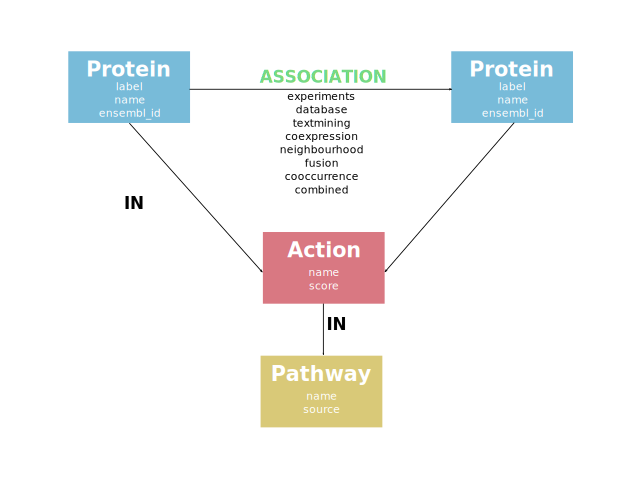
\includegraphics[width=0.9\linewidth]{database_scheme.png}
\end{figure}
\end{frame}

\begin{frame}{Workflow}
\begin{figure}
    \centering
    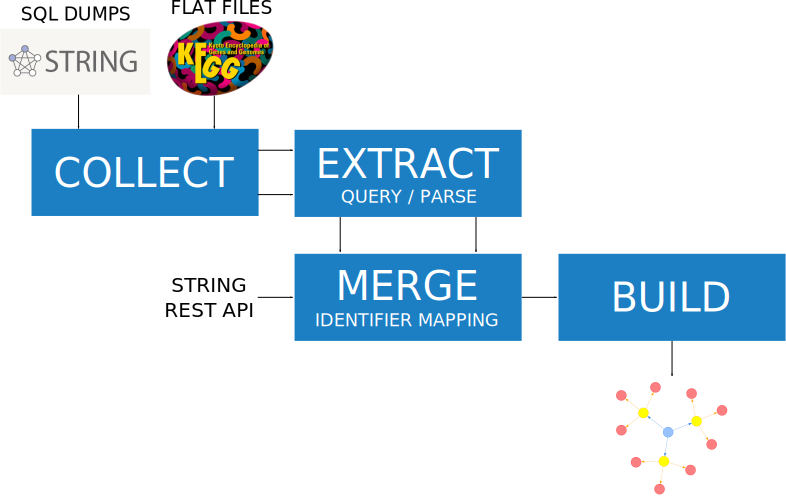
\includegraphics[width=0.9\linewidth]{workflow2.png}
\end{figure}
\end{frame}

\section{Results}

\definecolor{protein}{HTML}{178ab7}
\definecolor{disease}{HTML}{15a52f}
\definecolor{compound}{HTML}{8f17b7}

\begin{frame}{Cytokine Graph DB in numbers}
\begin{itemize}
    \item Cytokine-cytokine receptor interaction - Human (Homo sapiens)
    \vfill
    \item Nodes
    \begin{itemize}
        \item \textcolor{protein}{Protein}: 282
        \item \textcolor{orange}{Pathway}: 325
        \item \textcolor{red}{Drug}: 3 731
        \item \textcolor{disease}{Disease}: 969
        \item \textcolor{compound}{Compound}: 3 465
        \item \textcolor{gray}{Class}: 49
    \end{itemize}
    \vfill
    \item Relationships
    \begin{itemize}
        \item \textbf{ASSOCIATION}: 13 900
        \item \textbf{IN}: 17 752
    \end{itemize}
\end{itemize}
\end{frame}

%------------------------------------------------

\begin{frame}
\centering
\huge{(demo)}
\end{frame}

\section{Next steps}
\begin{frame}{Next steps}
\begin{itemize}
    \item Extend the database
    \begin{itemize}
        \item Protein - protein actions
        \item \href{https://www.genome.jp/kegg/drug/}{KEGG DRUG}
        \item \href{https://www.genome.jp/kegg/disease/}{KEGG DISEASE}
        \item \href{https://www.genome.jp/kegg/compound/}{KEGG COMPOUND}
    \end{itemize}
    \vfill
    \item Other species
    \vfill
    \item All proteins
    \vfill
    \item Web server
    \vfill
    \item Machine learning
\end{itemize}
\end{frame}

\begin{frame}
\centering
\huge{Thanks :)}
\bigskip \\
\small{
    \href{https://backofenlab.github.io/cytokine-graph-db/}{https://backofenlab.github.io/cytokine-graph-db/} \\
    \href{https://github.com/BackofenLab/cytokine-graph-db}{https://github.com/BackofenLab/cytokine-graph-db}
}
\end{frame}

\end{document}